
% ----------------------------------------------------------------------
%                   LATEX TEMPLATE FOR PhD THESIS
% ----------------------------------------------------------------------

% based on Harish Bhanderi's PhD/MPhil template, then Uni Cambridge
% http://www-h.eng.cam.ac.uk/help/tpl/textprocessing/ThesisStyle/
% corrected and extended in 2007 by Jakob Suckale, then MPI-CBG PhD programme
% and made available through OpenWetWare.org - the free biology wiki


%: Style file for Latex
% Most style definitions are in the external file PhDthesisPSnPDF.
% In this template package, it can be found in ./Latex/Classes/
\documentclass[twoside,11pt]{Latex/Classes/PhDthesisPSnPDF}


%: Macro file for Latex
% Macros help you summarise frequently repeated Latex commands.
% Here, they are placed in an external file /Latex/Macros/MacroFile1.tex
% An macro that you may use frequently is the figuremacro (see introduction.tex)
% This file contains macros that can be called up from connected TeX files
% It helps to summarise repeated code, e.g. figure insertion (see below).

% todo macro
\usepackage{color}
\newcommand{\todo}[1]{\noindent\textcolor{red}{{\bf \{TODO}: #1{\bf \}}}}

\usepackage{xspace}
\newcommand{\googleplus}{Google\nolinebreak\hspace{0em}\raisebox{.28ex}{\tiny\bf +}\kern-0.2ex\xspace}

% insert a centered figure with caption and description
% parameters 1:filename, 2:title, 3:description and label
\newcommand{\figuremacro}[3]{
	\begin{figure}[htbp]
		\centering
		\includegraphics[width=1\textwidth]{#1}
		\caption[#2]{\textbf{#2} - #3}
		\label{fig:#1}
	\end{figure}
}

% insert a centered figure with caption and description AND WIDTH
% parameters 1:filename, 2:title, 3:description and label, 4: textwidth
% textwidth 1 means as text, 0.5 means half the width of the text
\newcommand{\figuremacroW}[4]{
	\begin{figure}[htbp]
		\centering
		\includegraphics[width=#4\textwidth]{#1}
		\caption[#2]{\textbf{#2} - #3}
		\label{fig:#1}
	\end{figure}
}

% inserts a figure with wrapped around text; only suitable for NARROW figs
% o is for outside on a double paged document; others: l, r, i(inside)
% text and figure will each be half of the document width
% note: long captions often crash with adjacent content; take care
% in general: above 2 macro produce more reliable layout
\newcommand{\figuremacroN}[3]{
	\begin{wrapfigure}{o}{0.5\textwidth}
		\centering
		\includegraphics[width=0.48\textwidth]{#1}
		\caption[#2]{{\small\textbf{#2} - #3}}
		\label{fig:#1}
	\end{wrapfigure}
}

% predefined commands by Harish
\newcommand{\PdfPsText}[2]{
  \ifpdf
     #1
  \else
     #2
  \fi
}

\newcommand{\IncludeGraphicsH}[3]{
  \PdfPsText{\includegraphics[height=#2]{#1}}{\includegraphics[bb = #3, height=#2]{#1}}
}

\newcommand{\IncludeGraphicsW}[3]{
  \PdfPsText{\includegraphics[width=#2]{#1}}{\includegraphics[bb = #3, width=#2]{#1}}
}

\newcommand{\InsertFig}[3]{
  \begin{figure}[!htbp]
    \begin{center}
      \leavevmode
      #1
      \caption{#2}
      \label{#3}
    \end{center}
  \end{figure}
}


%%% Local Variables: 
%%% mode: latex
%%% TeX-master: "~/Documents/LaTeX/CUEDThesisPSnPDF/thesis"
%%% End: 




%: ----------------------------------------------------------------------
%:                  TITLE PAGE: name, degree,..
% ----------------------------------------------------------------------
% below is to generate the title page with crest and author name

%if output to PDF then put the following in PDF header
\ifpdf  
    \pdfinfo { /Title  (PhD and MPhil Thesis Classes)
               /Creator (TeX)
               /Producer (pdfTeX)
               /Author (YourName your@email.net)
               /CreationDate (D:YYYYMMDDhhmmss)  %format D:YYYYMMDDhhmmss
               /ModDate (D:YYYYMMDDhhmm)
               /Subject (xyz)
               /Keywords (add, your, keywords, here) }
    \pdfcatalog { /PageMode (/UseOutlines)
                  /OpenAction (fitbh)  }
\fi


\title{Enriching unstructured media content about events to enable semi-automated summaries, compilations, and improved search by leveraging social networks}



% ----------------------------------------------------------------------
% The section below defines www links/email for author and institutions
% They will appear on the title page of the PDF and can be clicked
\ifpdf
  \author{\href{mailto:tsteiner@lsi.upc.edu}{Thomas Steiner}}
%  \cityofbirth{born in XYZ} % uncomment this if your university requires this
%  % If city of birth is required, also uncomment 2 sections in PhDthesisPSnPDF
%  % Just search for the "city" and you'll find them.
  \collegeordept{\href{http://www.lsi.upc.edu/}{Departament de Llenguatges i Sistemes Informàtics}}
  \university{\href{http://www.upc.edu/}{Universitat Politècnica de Catalunya}}

  % The crest is a graphics file of the logo of your research institution.
  % Place it in ./frontmatter/figures and specify the width
  \crest{
\includegraphics[width=4cm]{upc-logo}}
  
% If you are not creating a PDF then use the following. The default is PDF.
\else
  \author{Thomas Steiner}
%  \cityofbirth{born in XYZ}
  \collegeordept{Departament de Llenguatges i Sistemes Informàtics}
  \university{Universitat Politècnica de Catalunya}
  \crest{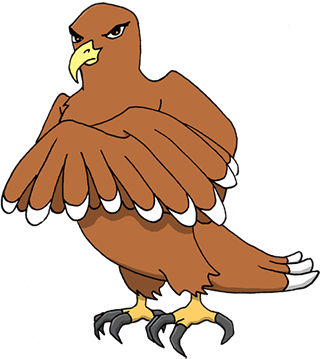
\includegraphics[width=4cm]{logo}}
\fi

%\renewcommand{\submittedtext}{change the default text here if needed}
\degree{Philosophi{\ae} Doctor (PhD)}
\degreedate{December 2012}


% ----------------------------------------------------------------------
       
% turn of those nasty overfull and underfull hboxes
\hbadness=10000
\hfuzz=50pt


%: --------------------------------------------------------------
%:                  FRONT MATTER: dedications, abstract,..
% --------------------------------------------------------------

\begin{document}

%\language{english}

% sets line spacing
\renewcommand\baselinestretch{1.2}
\baselineskip=18pt plus1pt


%: ----------------------- generate cover page ------------------------

\maketitle  % command to print the title page with above variables


%: ----------------------- cover page back side ------------------------
% Your research institution may require reviewer names, etc.
% This cover back side is required by Dresden Med Fac; uncomment if needed.

\newpage
\vspace{10mm}
1. Reviewer: Joaquim Gabarró Vallés (UPC)

\vspace{10mm}
2. Reviewer: Michael Hausenblas (DERI)

\vspace{20mm}
Day of the defense: \todo{add date of the defense}

\vspace{20mm}
\hspace{70mm}Signature from head of PhD committee:



%: ----------------------- abstract ------------------------

% Your institution may have specific regulations if you need an abstract and where it is to be placed in the document. The default here is just after title.

\begin{abstracts}

\textbf{(i) Mobile devices and social networks are omnipresent}

Mobile devices such as smartphones, tablets, or digital cameras
together with social networks enable people to create,
share, and consume enormous amounts of media items
like videos or photos both on the road or at home.
Such mobile devices---by pure definition---accompany
their owners almost wherever they may go.
In consequence, mobile devices are omnipresent
at all sorts of events to capture noteworthy moments.
Exemplary events can be keynote speeches at conferences,
music concerts in stadiums,
or even natural catastrophes like earthquakes
that affect whole areas or countries.
At such events---given a~stable network connection---part of
the event-related media items are published on social networks
both as the event happens or afterwards,
once a~stable network connection has been established again.

\textbf{(ii) Finding representative media items
for an event is hard}

Common media item search operations,
for example, searching for \emph{the} official video clip
for a~certain hit record on an online video platform
can in the simplest case be achieved based on potentially
shallow human-generated metadata
or based on more profound content analysis techniques
like optical character recognition,
automatic speech recognition,
or acoustic fingerprinting.
More advanced scenarios, however, like retrieving all
(or just the most representative) media items
that were created at a~given event
with the objective of creating \emph{event summaries} or
\emph{media item compilations} covering the event in question
are hard, if not impossible, to fulfill at large scale.
The main research question of this thesis
can be formulated as follows.

\textbf{(iii) Research question}

\textit{``Can user-customizable media galleries
that summarize given events be\linebreak
created solely based on textual and multimedia data
from social networks?''}

\textbf{(iv) Contributions}

In the context of this thesis, we have developed and evaluated
a~novel interactive application and related methods
for media item enrichment,
leveraging social networks, utilizing the Web of Data,
techniques known from Content-based Image Retrieval~(CBIR)
and Content-based Video Retrieval~(CBVR),
and fine-grained media item addressing schemes
like Media Fragments URIs
to provide a~scalable and near realtime solution
to realize the abovementioned scenario
of event summarization and media item compilation.

\textbf{(v) Methodology}

For any event with given event title(s),
(potentially vague) event location(s), and
(arbitrarily fine-grained) event date(s),
our approach can be divided in the following six steps.

\begin{enumerate}
  \item Via the textual search APIs (Application Programming Interfaces) of
        different social networks,
        we retrieve a~list of potentially event-relevant
        microposts that either contain media items directly,
        or that provide links to media items
        on external media item hosting platforms.
  \item Using third-party
        Natural Language Processing (NLP) tools,
        we recognize and disambiguate named entities
        in microposts to predetermine their relevance.
  \item We extract the binary media item data
        from social networks or media item hosting platforms
        and relate it to the originating microposts.
  \item Using CBIR and CBVR techniques, we first deduplicate
        exact-duplicate and near-duplicate media items
        and then cluster similar media items.
  \item We rank the deduplicated and clustered list
        of media items and their related microposts
        according to well-defined ranking criteria.
  \item In order to generate interactive and user-customizable
        media galleries that visually and audially summarize the
        event in question, we compile the top-$n$ ranked
        media items and microposts in aesthetically pleasing
        and functional ways.
\end{enumerate}
\end{abstracts}


% The original template provides and abstractseparate environment, if your institution requires them to be separate. I think it's easier to print the abstract from the complete thesis by restricting printing to the relevant page.
% \begin{abstractseparate}
%   \begin{abstracts}

\textbf{(i) Mobile devices and social networks are omnipresent}

Mobile devices such as smartphones, tablets, or digital cameras
together with social networks enable people to create,
share, and consume enormous amounts of media items
like videos or photos both on the road or at home.
Such mobile devices---by pure definition---accompany
their owners almost wherever they may go.
In consequence, mobile devices are omnipresent
at all sorts of events to capture noteworthy moments.
Exemplary events can be keynote speeches at conferences,
music concerts in stadiums,
or even natural catastrophes like earthquakes
that affect whole areas or countries.
At such events---given a~stable network connection---part of
the event-related media items are published on social networks
both as the event happens or afterwards,
once a~stable network connection has been established again.

\textbf{(ii) Finding representative media items
for an event is hard}

Common media item search operations,
for example, searching for \emph{the} official video clip
for a~certain hit record on an online video platform
can in the simplest case be achieved based on potentially
shallow human-generated metadata
or based on more profound content analysis techniques
like optical character recognition,
automatic speech recognition,
or acoustic fingerprinting.
More advanced scenarios, however, like retrieving all
(or just the most representative) media items
that were created at a~given event
with the objective of creating \emph{event summaries} or
\emph{media item compilations} covering the event in question
are hard, if not impossible, to fulfill at large scale.
The main research question of this thesis
can be formulated as follows.

\textbf{(iii) Research question}

\textit{``Can user-customizable media galleries
that summarize given events be\linebreak
created solely based on textual and multimedia data
from social networks?''}

\textbf{(iv) Contributions}

In the context of this thesis, we have developed and evaluated
a~novel interactive application and related methods
for media item enrichment,
leveraging social networks, utilizing the Web of Data,
techniques known from Content-based Image Retrieval~(CBIR)
and Content-based Video Retrieval~(CBVR),
and fine-grained media item addressing schemes
like Media Fragments URIs
to provide a~scalable and near realtime solution
to realize the abovementioned scenario
of event summarization and media item compilation.

\textbf{(v) Methodology}

For any event with given event title(s),
(potentially vague) event location(s), and
(arbitrarily fine-grained) event date(s),
our approach can be divided in the following six steps.

\begin{enumerate}
  \item Via the textual search APIs (Application Programming Interfaces) of
        different social networks,
        we retrieve a~list of potentially event-relevant
        microposts that either contain media items directly,
        or that provide links to media items
        on external media item hosting platforms.
  \item Using third-party
        Natural Language Processing (NLP) tools,
        we recognize and disambiguate named entities
        in microposts to predetermine their relevance.
  \item We extract the binary media item data
        from social networks or media item hosting platforms
        and relate it to the originating microposts.
  \item Using CBIR and CBVR techniques, we first deduplicate
        exact-duplicate and near-duplicate media items
        and then cluster similar media items.
  \item We rank the deduplicated and clustered list
        of media items and their related microposts
        according to well-defined ranking criteria.
  \item In order to generate interactive and user-customizable
        media galleries that visually and audially summarize the
        event in question, we compile the top-$n$ ranked
        media items and microposts in aesthetically pleasing
        and functional ways.
\end{enumerate}
\end{abstracts}

% \end{abstractseparate}


%: ----------------------- tie in front matter ------------------------

\frontmatter
\begin{dedication} %this creates the heading for the dedication page
To Laura, Lena, Emma, and Nil.
\end{dedication}

\begin{acknowledgements}

\textbf{Personal Acknowledgements:}

First and foremost, I~would like to thank my wife Laura
for her support, understanding, patience, and energy
during my time as a~PhD student, and simply for being at my side.
Without you, I~would not be where I~am today.

I~wholeheartedly thank my two advisors Joaquim Gabarró Vallés
and Michael Hausenblas for their guidance, helpful comments,
informative pointers, and especially
for their constructive criticisms.
The areas of research that I~have tackled in this thesis
are still young and sometimes uncharted territory.
I~am very thankful that the two of you have ventured
on the undertaking of leading me through this thesis.

I~deeply appreciate all the review comments, thoughts, challenging questions,
and, last not least, the \LaTeX~help of my dear friend
and research colleague Ruben Verborgh.
It was, is, and will be an honor to work with you.
My warm thanks also go to Raphaël Troncy and his team
at \mbox{EURECOM} Sophia Antipolis in France
who have helped shape some of the ideas presented in this thesis.

I~would like to thank my former and current managers at Google,
namely N.~Kryvossidis, R.~Ashley, C.~Bouchère, and I.~Sassarini
for their support for my thesis.
A~lot of valuable input for my thesis came in via social networks.
My thanks go out to everyone I have interacted with
around the hashtag \texttt{\#TomsPhD}
on Twitter, \googleplus, and Facebook.

Finally, I~sincerely thank my parents and my brother
who have made me the person I~am today.
My parents have taught me
not to go for the easy choices, even
if at times they may seem tempting,
but instead to try harder and never give up.
This thesis also is for you.

\textbf{Formal Acknowledgements:}

The research presented in this thesis
was partially supported by the European Commission
under Grant No. 248296 with the European Union (FP7 ICT STReP)
project \mbox{\emph{I-SEARCH}}.

\vspace{80mm}

\textbf{To cite this document:}

\small
\begin{verbatim}
  @phdthesis{steiner2013thesis,
    author = {Thomas Steiner},
    title  = {Enriching Unstructured Media Content About Events to
              Enable Semi-Automated Summaries, Compilations, and
              Improved Search by Leveraging Social Networks},
    year   = {2013},
    school = {Universitat Polit\`{e}cnica de Catalunya}
  }
\end{verbatim}

\normalsize

\vspace{10mm}
\textbf{Copyright and License:}\\\\
\small \copyright \normalsize 2013 Thomas Steiner\\
Licensed under the Creative Commons Attribution-ShareAlike 3.0 License.\\
\url{http://creativecommons.org/licenses/by-sa/3.0/}

\end{acknowledgements}



%: ----------------------- contents ------------------------

\setcounter{secnumdepth}{3} % organisational level that receives a numbers
\setcounter{tocdepth}{3}    % print table of contents for level 3
\tableofcontents            % print the table of contents
% levels are: 0 - chapter, 1 - section, 2 - subsection, 3 - subsection


%: ----------------------- list of figures/tables ------------------------

\listoffigures	% print list of figures

\listoftables  % print list of tables


%: ----------------------- glossary ------------------------

% Tie in external source file for definitions: /frontmatter/glossary.tex
% Glossary entries can also be defined in the main text. See glossary.tex
% this file is called up by thesis.tex
% content in this file will be fed into the main document

% Glossary entries are defined with the command \nomenclature{1}{2}
% 1 = Entry name, e.g. abbreviation; 2 = Explanation
% You can place all explanations in this separate file or declare them in the middle of the text. Either way they will be collected in the glossary.

% required to print nomenclature name to page header
\markboth{\MakeUppercase{\nomname}}{\MakeUppercase{\nomname}}

\nomenclature{NLP}{Natural Language Processing}
\nomenclature{CBIR}{Content-based Image Retrieval} 
\nomenclature{CBVR}{Content-based Video Retrieval} 
\nomenclature{RDF}{Resource Description Framework}
\nomenclature{W3}{World-Wide Web}
\nomenclature{WWW}{World-Wide Web}
\nomenclature{CERN}{European Organization for Nuclear Research}
\nomenclature{HTML}{Hypertext Markup Language}
\nomenclature{URI}{Unique Resource Identifier}
\nomenclature{URL}{Unique Resource Locator}
\nomenclature{JSON}{JavaScript Object Notation}
\nomenclature{Turtle}{Terse RDF Triple Language}
\nomenclature{CURIE}{Compact URI}
\nomenclature{SPARQL}{SPARQL Protocol and RDF Query Language}
\nomenclature{W3C}{World Wide Web Consortium}
\nomenclature{LOD}{Linking Open Data}
\nomenclature{SNS}{Social Network(ing) Site}
\nomenclature{API}{Application Programming Interface}
\nomenclature{NEE}{Named Entity Extraction}
\nomenclature{NER}{Named Entity Recognition}
\nomenclature{OWL}{Web Ontology Language}
\nomenclature{DOM}{Document Object Model}
\nomenclature{POS}{Part-of-Speech (tagging)} 

\begin{multicols}{2} % \begin{multicols}{#columns}[header text][space]
\begin{footnotesize} % scriptsize(7) < footnotesize(8) < small (9) < normal (10)

\printnomenclature[1.5cm] % [] = distance between entry and description
\label{nom} % target name for links to glossary

\end{footnotesize}
\end{multicols}



%: --------------------------------------------------------------
%:                  MAIN DOCUMENT SECTION
% --------------------------------------------------------------

% the main text starts here with the introduction, 1st chapter,...
\mainmatter

\renewcommand{\chaptername}{} % uncomment to print only "1" not "Chapter 1"


%: ----------------------- subdocuments ------------------------

% Parts of the thesis are included below. Rename the files as required.
% But take care that the paths match. You can also change the order of appearance by moving the include commands.

\chapter{Event Summarization Challenge}
\label{cha:introduction}

% the code below specifies where the figures are stored
\ifpdf
    \graphicspath{{1_introduction/figures/PNG/}{1_introduction/figures/PDF/}{1_introduction/figures/}}
\else
    \graphicspath{{1_introduction/figures/EPS/}{1_introduction/figures/}}
\fi

\section{Motivation and Problem Statement}

A~very open definition of the word \emph{event}
given by WordNet~\cite{fellbaum1998wordnet,miller1995wordnet} is
\emph{``something that happens at a~given place and time''}.
Following this definition,
we are indeed surrounded by events,
most of which are of little to no interest for us.
A~concert somewhere in the world of a~band
that we do not even know may be a~good example.
For some events, however, we may care more, for example,
a~concert of a~band that we know and like,
even if it takes place at a~location far away from us.
Finally, for very few events, we may care a~lot,
maybe even enough to physically attend the event,
like a~concert of our favorite band
if it takes place in our city, is not sold out,
and not too expensive.

All this motivates the need for \emph{event summarization}.
If there is an event that we could not attend
for any given reason,
but that we are interested in,
a~good event summarization can help us get a~feeling
for the event's atmosphere.
Similarly, if there is an event that we attended,
we can revive the event's most fascinating moments
based on the event summarization.

A~\emph{media gallery} in the context of
our event summarization task is
a~\emph{best-of} compilation of photos, videos,
and microposts retrieved from social networks
that are related to a~given event.
Event summarization covers textual
as well as multimedia content.
We say a~media gallery is of high quality,
if it fulfills the following properties.

\begin{enumerate}
  \item \textit{Conciseness:}
        it conveys a~lot of information clearly
        and in few media items.
  \item \textit{Comprehensiveness:}
        it is complete and covers all representative
        elements or aspects of an event.
  \item \textit{Authenticity:}
        it is of undisputed origin and genuine.
  \item \textit{Diversity:}
        it shows a~great deal of variety.
  \item \textit{Interestingness:}
        it catches and holds the attention of the viewer.     
\end{enumerate}

\section{Research Question and Hypothesis}

The main research question for this thesis
can be formulated as follows.
 
\textit{``Can user-customizable
media galleries that summarize given events be
created solely based on textual and multimedia data
from social networks?''}

\noindent The hypothesis that we test in this thesis
can be formulated as follows.

We argue that through media galleries that leverage content
that was shared on social networks,
a~more \emph{authentic}, more \emph{concise},
more \emph{comprehensive}, more \emph{diverse},
and also more \emph{interesting}
view on events gets possible than by limiting oneself
to officially produced media content;
and that further such media galleries can be generated
more \emph{efficiently} and \emph{in shorter time}
than manually produced media galleries.

We validate these subjective and objective
criteria with experiments for events of different categories
such as sports, politics, culture, leisure,
music, conferences, \emph{etc.}

\section{Approach}

The objective of this thesis is the development
of methods for the automated summarization of events
based on media items shared on social networks.
A~schematic overview of the approach can be seen
in~\autoref{fig:thesis-diagram}.
As an event takes places and shortly thereafter
(symbolized by the timeline marked with \emph{2h Event}),
people share media items related to the event
on multiple social networks
(symbolized by the photo and video pictograms
above the event timeline).
Via the textual search APIs (Application Programming Interfaces)
of these different social networks,
we retrieve a~list of potentially event-relevant
microposts that either contain media items directly,
or that provide links to media items
on external media item hosting platforms.
Using third-party NLP tools,
we recognize and disambiguate named entities
in the microposts to predetermine their relevance.
We extract the binary media item data
from social networks or media item hosting platforms
and relate it to the originating microposts
(symbolized by the central cloud).
Using CBIR and CBVR techniques, we first deduplicate
duplicate and near-duplicate media items,
and then cluster similar media items
(symbolized by the green, red, and orange markers).
We rank the deduplicated and clustered list
of media items and their related microposts
according to well-defined ranking criteria.
In order to generate interactive and user-customizable
media galleries that visually and audially summarize the
event in question, we compile the top-$n$ ranked
media items and microposts in an aesthetic way
(symbolized by the timeline marked with \emph{5min Summary}).

\begin{figure}[!ht]
  \centering
  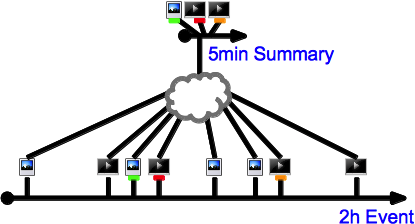
\includegraphics[]{thesis-diagram.png}
  \caption[Schematic depiction of event summary generation]
    {Schematic depiction of event summary generation
    based on deduplicated, clustered, and ranked media items
    for an exemplary event}
  \label{fig:thesis-diagram}
\end{figure}

\section{Contributions}

In this thesis, we report on methods for
the automated generation of event summaries.
This particular field of research touches on many related areas
of research and research communities,
amongst which social network research, multimedia content analysis,
Semantic Web and Natural Language Processing (NLP),
human factors in computing systems,
and Web services.
Early on in the process of this thesis,
we have sought and incorporated expert feedback based on
a~Doctoral Consortium paper~%
\cite{steiner2011enrichingunstructured}.
We have broken our contributions down into
the following topics.

\subsection{Social Network Multimedia and Data Analysis}

We have worked on methods for the aggregation, extraction,
deduplication, clustering, and compilation
of social media contents from
multiple social networks~%
\cite{rizzo2012whatfresh}.
Those methods were applied and evaluated
for the enhancement of conference experiences~%
\cite{khrouf2012aggregatingsocialmedia,khrouf2012confomaton}.

\subsection{Application of Semantic Web and NLP Techniques}

In order to make sense out of social network microposts,
we have worked on methods to consolidate and rank
the results of multiple named entity recognition and
disambiguation APIs and to track their data provenance~%
\cite{steiner2011addingmeaning}.
We have applied and evaluated those methods
for the consumer-oriented detection of trending microposts
on a~major commercial social network~%
\cite{steiner2011tweetconsumers}.


\subsection{Video Content and Metadata Analysis}

We have worked on methods for named entity extraction and
disambiguation for online videos based on closed captions
and other textual metadata, which make online video
more accessible, searchable, and interconnected~%
\cite{steiner2010semwebvid,steiner2010semwebvidchallenge}.
Further, we have combined those textual methods with 
video content analysis methods for the on-the-fly detection
of shot boundaries for online videos~%
\cite{steiner2012shotdetection}.
We have defined aesthetic principles
for the automated generation of media gallery layouts
for visual and audial event summarization
based on social network multimedia data~%
\cite{steiner2012definingaesthetic}.
        
\subsection{Crowdsourcing}

The video content analysis methods mentioned before
were combined with methods for the crowdsourced detection
of events in online videos~%
\cite{steiner2011crowdsourcingevent}.
We have further worked on crowdsourcing methods
for the extraction of knowledge items from arbitrary Web pages~%
\cite{steiner2012sekiathome,steiner2012sekiathomechallenge}.

\subsection{Studies}

We have contributed an examination of Linked Data usage and
visualization techniques of a~major commercial search engine~%
\cite{steiner2010howgoogleisusing}.
In addition to that, we have studied the usefulness and relevance
of social network updates which were added to search engine
results pages (SERP) of a~major commercial search engine~%
\cite{steiner2012addingrealtime}.

\subsection{Multimodal Search Engines}

We have worked on an examination of context-aware querying
for multimodal search engines~%
\cite{etzold2012contextawarequerying,steiner2012isearch}.
Further, we have studied user interface constraints on
mobile and desktop devices for a~multimodal search engine
and demonstrated that those constraints can be overcome~%
\cite{steiner2012onesizedoesnotfitall}.


\subsection{Web Service Description}

We have worked on methods for the semantic description of Web APIs,
their discoverability, their automated consumption,
their semantic interlinking, and their social aspects~%
\cite{verborgh2011descriptionandinteraction,verborgh2011efficientruntime,verborgh2011integratingdata,verborgh2012capturingthefunctionality,verborgh2012functionalcomposition,verborgh2012functionaldescriptions,verborgh2012missinglinks,verborgh2012restdesc,verborgh2012socialdescriptionrevolution}.
We have studied the feasibility of truly RESTful behavior
for Web APIs in the sense of Dr. Roy Fielding~%
\cite{steiner2011fulfilling}.
        
\subsection{Standardization and Specifications}        
We have helped to shape a~W3C specification on media
fragment addressing schemes for audio and video items~%
\cite{troncy2012mediafragments}.
Further, we have worked on the definition of a~unified framework
for the description of multimedia content objects~%
\cite{axenopoulos2012isearch,daras2011unifiedframework}.
Finally, we have contributed to a~white paper on the
Future Media Internet Architecture~%
\cite{alduan2011futureinternet}.

\subsection{Others}

We have developed methods for unobtrusively fixing
common annoyances on arbitrary Web pages~%
\cite{steiner2012xkcd37}.

\section{Thesis Structure}

The remainder of this thesis is structured as follows. 

\autoref{cha:background} introduces the Semantic Web and its technologies.
Starting from the non-semantic Web,
we show how structured data can be added to Web pages
and briefly present DBpedia as a~knowledge base
founded on structured data extracted from Wikipedia.
We then continue with the Resource Description Framework
and explain how it represents facts with triples.
We provide examples of RDF's different serialization formats.
Afterwards, we outline the Semantic Web vision of
a~global giant database and present the Semantic Web
query language SPARQL.
We close the chapter with an introduction of Sir Tim Berners-Lee's
Linked Data principles and show how data publisher that publish
datasets according to those principles are visualized in the
Linking Open Data cloud.

\autoref{cha:social-networks}
\autoref{cha:micropost-annotation}
\autoref{cha:eventdetection}
\autoref{cha:media-item-extraction}
\autoref{cha:shot-boundary-detection}
\autoref{cha:media-item-deduplication}
\autoref{cha:media-item-ranking}
\autoref{cha:media-item-compilation}
\autoref{cha:future-work}

Each chapter is closed by a~final section called
\emph{Chapter Notes}, which contains references to publications
that the chapter is based upon,
and in some cases pointers to related material for further reading.

\bibliographystyle{plainnat}
\clearpage
\bibliography{backmatter/references}
	% background information

% --------------------------------------------------------------
%:                  BACK MATTER: appendices, refs,..
% --------------------------------------------------------------

% the back matter: appendix and references close the thesis


%: ----------------------- bibliography ------------------------

% The section below defines how references are listed and formatted
% The default below is 2 columns, small font, complete author names.
% Entries are also linked back to the page number in the text and to external URL if provided in the BibTex file.

% PhDbiblio-url2 = names small caps, title bold & hyperlinked, link to page 
\begin{multicols}{2} % \begin{multicols}{ # columns}[ header text][ space]
\begin{tiny} % tiny(5) < scriptsize(7) < footnotesize(8) < small (9)

\bibliographystyle{Latex/Classes/PhDbiblio-url2} % Title is link if provided
\renewcommand{\bibname}{References} % changes the header; default: Bibliography

\bibliography{backmatter/references} % adjust this to fit your BibTex file

\end{tiny}
\end{multicols}

% --------------------------------------------------------------
% Various bibliography styles exit. Replace above style as desired.

% in-text refs: (1) (1; 2)
% ref list: alphabetical; author(s) in small caps; initials last name; page(s)
%\bibliographystyle{Latex/Classes/PhDbiblio-case} % title forced lower case
%\bibliographystyle{Latex/Classes/PhDbiblio-bold} % title as in bibtex but bold
%\bibliographystyle{Latex/Classes/PhDbiblio-url} % bold + www link if provided

%\bibliographystyle{Latex/Classes/jmb} % calls style file jmb.bst
% in-text refs: author (year) without brackets
% ref list: alphabetical; author(s) in normal font; last name, initials; page(s)

%\bibliographystyle{plainnat} % calls style file plainnat.bst
% in-text refs: author (year) without brackets
% (this works with package natbib)


% --------------------------------------------------------------

%: Declaration of originality

% Thesis statement of originality -------------------------------------

% Depending on the regulations of your faculty you may need a declaration like the one below. This specific one is from the medical faculty of the university of Dresden.

\begin{declaration}        %this creates the heading for the declaration page

I herewith declare that I have produced this document without the prohibited assistance of third parties and without making use of aids other than those specified; notions taken over directly or indirectly from other sources have been identified as such. This document has not previously been presented in identical or similar form to any other examination board.

The thesis work was conducted from February 2010 to December 2012 under the supervision of Joaquim Gabarró Vallés (UPC Barcelona, Spain) and Michael Hausenblas (DERI Galway, Ireland).

\vspace{10mm}

Barcelona,


\end{declaration}


% ----------------------------------------------------------------------

\end{document}
